\section{Probabilidad de error en base a parámetros del canal} %Sistema completo de comunicación digital en banda base}

\begin{figure}[htb]
    \centering
    \resizebox{\textwidth}{!}{%
    \bpgf{Imagenes/digBB/digBB-1}
    \begin{blockdiagram}
        \matrix[row sep=5mm, column sep=10mm]{
            & & \node[etiqueta] (ruido) {\large ruido blanco, $\frac{\eta}{2}$}; & & & & & \node[punto] (p1) {}; & \node [punto] (p2) {};\\
            \node[etiqueta] (inicio) {\large  $\sum_k a_k p_T(t-kT_s)$}; %& \node[block] (pulso) {$P_T(t)$};
             & \node[block] (canal) {\large CANAL} node[above=3mm] {
                    \begin{minipage}{2.2cm}
                       \large  (ancho de banda $B$)
                    \end{minipage}};
            & \node[operator] (sum) {$+$}; & \node [block] (filtro) {\large $\hat{H}_R(f)$} node [below=5mm] {
            \begin{minipage}{2.5cm}
                FILTRO DE\\RECEPCI�N
                \end{minipage}};
            & \node[punto] (p3) {} node [anchor=south] {\large $x_R(t)+n(t)$}; & \node [punto] (p4) {}; & & & \node[punto] (p5) {}; & \node [draw, isosceles triangle,thick] (comp) {
            \begin{minipage}{5mm}
                $+$\\$-$
            \end{minipage}};
            & \node[etiqueta] (salida) {\large $\{\hat{a}_k\}$};\\
            & & & & & & \node[block] (sinc) {\large SINCR}; & & \node [etiqueta] (v0) {$A_0$};\\
        };
        \draw [-stealth] (inicio) -- (canal);
        \draw [-stealth] (canal) -- (sum);
        \draw [-stealth] (ruido) -- (sum);
        \draw [-stealth] (sum) -- (filtro);
        \draw (filtro) -- (p3) -- (p4) -- (p2);
        \draw [-stealth] (p3) |- (sinc);
        \draw [-stealth] (sinc) -| (p1);
        \draw [-stealth] (p5) |- (comp.150);
        \draw [-stealth] (v0) |- (comp.south west);
        \draw [-stealth] (comp) -- (salida);
    \end{blockdiagram}
\endpgfgraphicnamed

    }
\end{figure}

Se transmite una onda PAM por un canal de ancho de banda limitado
$B$, que además adiciona ruido. Al igual que en la comunicación
analógica, colocamos un filtro de recepción $\hat{H}_R(f)$ para
limitar el ruido en la detección. La salida de ese filtro va a la
etapa de detección recién estudiada. Tenemos entonces tres ondas
PAM:
\begin{itemize}
\item $x_T(t)= \sum_k a_k p_T(t-kT_s)$, la onda transmitida.
$p_T(t)$ es la forma de pulso seleccionada.
\item $x(t)=\sum a_k p(t-kT_s)$, la onda a la salida del canal,
a la que se superpone el ruido blanco. La forma de pulso $p(t)$
incorpora la distorsión del canal.
\item $x_R(t) = \sum_k a_k
p_R(t-kT_s)$, la onda a la salida del filtro de recepción, a la
que se superpone el ruido $n(t)$. \'Este tiene media nula y
varianza
\[\sigma^2=E[n(t)^2]=\frac{\eta}{2}\displaystyle\int^{+\infty}_{\infty}
|\hat{H}_R(f)|^2\d f.\]
\end{itemize}
Estudiamos el sistema completo distinguiendo según la forma de
pulso transmitida.

\begin{enumerate}
    \renewcommand\theenumi{\Roman{enumi}}
    \item \textbf{Comunicación con pulsos de Nyquist ideales}.
    \label{item:1}
    Es decir $p_T(t) = \sinc(\pi f_s t)$, con $f_s=2B$. \'Este es el caso más simple, donde la señal transmitida pasa sin distorsión por el
    canal:
 \[ p(t) = \sinc(\pi f_s t), \quad \hat{P}(f) = T_s
    p_{[-\frac{f_s}{2},\frac{f_s}{2}]}(f).\]
    En particular $x(t)$ está confinada a la banda $[-B,B]$. Para símbolos IID, de media $\mu$ y varianza
    $\sigma_a^2$, su densidad espectral de potencia es
    \begin{center}\begin{minipage}{\textwidth}
        \bpgf{Imagenes/digBB/digBB-2}
        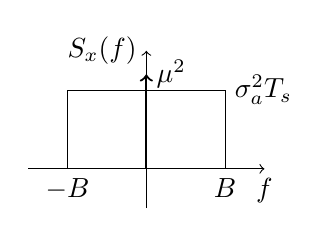
\begin{tikzpicture}
            \draw [->] (-1.5,0) -- (1.5,0) node [anchor=north] {$f$};
            \draw [->] (0,-0.5) -- (0,1.5) node [anchor=east] {$S_x(f)$};
            \draw (-1,0) node [anchor=north] {$-B$} -- (-1,1) -- (1,1) node [anchor=west] {$\sigma_a^2 T_s$} -- (1,0) node [anchor=north] {$B$};
            \draw [thick,->] (0,0) -- (0,1.2) node [anchor=west] {$\mu^2$};
        \end{tikzpicture}
        \endpgfgraphicnamed\end{minipage}
    \end{center}
    La potencia media de señal a la salida del canal es
     \[
     \langle x ^2 \rangle = \int_{-\infty}^\infty S_x(f)\d f =
     \mu^2 + \sigma_a^2 T_s 2B = \mu^2 + \sigma_a^2 = E[a_k^2].
     \]
     Notar que como $\|p\|^2 = \int_{-\infty}^\infty |\hat{P}(f)|^2 \d f = T_s$ se verifica en particular para este caso la f\'ormula
     anunciada en la sección anterior,
     \[\langle x^2 \rangle = E[a_k^2] \|p\|^2 f_s = \overline{E_p}
     f_s.\]
    $x(t)$ llega contaminada de ruido blanco. Resulta entonces
    natural en este caso proceder  como en el caso analógico, y poner como
    filtro de recepción simplemente un pasabajos ideal $[-B,B]$,
    que rechaza al ruido fuera de banda. Notar que:
    \begin{itemize}
    \item La señal de recepci\'on sigue intacta, $p_R(t) = p(t)$, es decir no hay ISI en la detecci\'on.
    \item El ruido de recepción tiene $\sigma^2=\eta B = \frac{\eta f_s}{2}$.
    \end{itemize}
%

    Calculamos ahora expresiones para la probabilidad de error de detección $P_e$ en términos de parámetros físicos del
    canal, para las codificaciones de línea polar o unipolar.

    \begin{description}
        \item[Caso polar binario] $a_k=\pm A$, umbral \'optimo
        $A_0=0$, $\langle x^2 \rangle = A^2$.
        \[ \Rightarrow \ \ P_e = Q\left(\frac{A}{\sigma}\right) = Q\left(\sqrt{\frac{\langle x^2 \rangle}{\sigma^2}}\right) = Q\left(\sqrt{\frac{S}{N}}\right).\]
        que es la misma expresión que obtuvimos con pulsos NRZ.

        Otra expresión (más fácil de generalizar): sea $\overline{E}_p$ la energía media del pulso $a_k
        p(t)$,
        en este caso $\overline{E}_p = E[a_k^2]\|p\|^2 = A^2 T_s$.
                \[\left.\begin{gathered}
                        A^2 = S = \overline{E}_p f_s\\
                        \sigma^2 = N = \eta \frac{f_s}{2}
                      \end{gathered}\right\}\Rightarrow \frac{S}{N} = \frac{2\overline{E}_p}{\eta}\Rightarrow \col{P_e = Q\left(\sqrt{\frac{2\overline{E}_p}{\eta}}\right)}\]
        que depende solo de parámetros físicos del canal:
        \begin{itemize}
            \item Energía media del pulso.
            \item Densidad espectral de ruido.
            \item ¡No depende de $f_s$!
        \end{itemize}
        \vspace{1ex}

        \item[Caso unipolar binario] $a_k = \{0,A\}$, umbral \'optimo
        $A_0=\frac{A}{2}$, $\langle x^2 \rangle = S = \frac{A^2}{2}$.
       % Entonces $S_x(f) = \sigma^2 f_s |\hat{P}(f)|^2 + \mu^2 f_s^2 \hat{P}(f)^2 = \frac{A^2}{4} T_s p_{[-\frac{f_s}{2},\frac{f_s}{2}]}(f) + \frac{A^2}{4}\delta(f)$
        \begin{align*}
 %           S = \langle x^2 \rangle = \frac{A^2}{4} + \frac{A^2}{4} = \frac{A^2}{2}\\
         \sigma^2 = N = \eta \frac{f_s}{2} \Longrightarrow   P_e = Q\left(\frac{A}{2\sigma}\right) =
         Q\left(\frac{1}{\sqrt{2}}\sqrt{\frac{S}{N}}\right).
        \end{align*}

        También aqúi tenemos $\frac{S}{N} = \frac{2\overline{E}_p}{\eta}$
%        \overline{E}_p = E[a_k^2] \int p(t)^2\d t = \frac{A^2}{2} T_s\Rightarrow S = \overline{E}_p T_s$, $N=\frac{\eta f_s}{2}$
        \[\Rightarrow \col{P_e = Q\left(\sqrt{\frac{\overline{E}_p}{\eta}}\right)}\]
        que es menos eficiente que el caso polar.
    \end{description}

\newpage


    \item \textbf{Pulsos de Nyquist de exceso de ancho de banda $\alpha$.}
    \label{item:2}
    Para que estos pulsos pasen intactos por el canal, se require
    la relación $f_s (1+\alpha) \leq 2B$, más restrictiva que la
    anterior. Suponiendo que esto ocurre, podemos usar la misma
    estrategia para elegir el filtro: dejar el pulso intacto,
    eliminar el ruido fuera de banda. Por tanto,
 \[
\Rightarrow \sigma^2 = \frac{\eta f_s}{2}(1+\alpha).
\]
Aquí no buscamos expresiones en términos de $\frac{S}{N}$, en
particular la f\'ormula sencilla para la potencia de la señal PAM
no se aplica. Generalizamos las expresiones para la probabilidad
de error en términos de $\frac{\overline{E}_p}{\eta}$. La energía
media del pulso es
    \[\overline{E}_p = E[a_k^2] \int p(t)^2\d t = E[a_k^2] T_s \left(\underbrace{\frac{1}{T_s}\int |\hat{P}(f)|^2\d f}_{\text{llamamos }\beta}\right)
     = \beta E[a_k^2] T_s.\]
    Se puede verificar (usando la desigualdad de Cauchy-Schwarz) que el parámetro $\beta$ cumple  $\frac{1}{1+\alpha} \leq \beta \leq
    1$.

    Para el caso polar binario, $\overline{E}_p = \beta A^2 T_s\Rightarrow A=\sqrt{\overline{E}_p \frac{f_s}{\beta}}$. $\sigma=\sqrt{\dfrac{\eta f_s}{2} (1+\alpha)}$.

    \[\Rightarrow P_e = Q\left(\frac{A}{\sigma}\right) = Q\left(\sqrt{\frac{2\overline{E}_p}{\eta (1+\alpha)\beta}}\right).\]
    Se agregó un factor $\beta(1+\alpha)\geq 1$ en el denominador,
    respecto del caso de pulsos de Nyquist ideales. Esto deteriora
    $P_e$. Lo mismo ocurre en el caso unipolar.

    Intuitivamente: tuvimos que ensanchar el filtro para dejar pasar la señal y no introducir ISI, pero esta no tiene ``tanta fuerza'' en la parte alta de la banda.

    \item \textbf{Caso de pulsos rectangulares RZ o NRZ}
    \label{item:3}

    Supongamos que el canal tiene $B$ grande y los pulsos $p(t)$ llegan esencialmente rectangulares, ¿qué hago con $H_R$? El dilema es:
    \begin{itemize}
        \item Filtro muy ancho, no deforma pulsos pero pasa mucho ruido a la etapa de
        detecci\'on.
        \item Filtro angosto, reduce el ruido pero deforma los pulsos, introduce ISI.
    \end{itemize}
    Para este tipo de pulsos la estrategia de ``dejarlos pasar intactos'', que tomamos de la comunicación analógica, no
    es la apropiada.
    En realidad, aqu\'i no importa dejar la onda intacta sino lograr la máxima amplitud en el momento del
    muestreo, en relaci\'on al ruido. La optimización del filtro de
    detecci\'on para estos fines se verá a continuación.
\end{enumerate}
